\documentclass[11pt]{standalone}
\usepackage{amssymb}
\usepackage{amsmath}
\usepackage[no-math]{fontspec}
\usepackage{unicode-math}
\setmainfont{Libertinus Sans}
\setsansfont{Libertinus Sans}
\setmathfont{Libertinus Math}
\usepackage{pgf,xcolor}
\usepackage{tikz}
\usetikzlibrary{arrows.meta, backgrounds, calc}
\usepackage{pgfplots}
\pgfplotsset{compat=newest}
\usepackage{pifont}

\definecolor{my_darkgray}{HTML}{484949}
\definecolor{my_lightgray}{HTML}{F3F4F4}
\definecolor{my_darkblue}{HTML}{005A94}
\definecolor{my_lightblue}{HTML}{CCDEE9}
\definecolor{my_yellow}{HTML}{FFEC7F}
\definecolor{my_red}{HTML}{E60000}
\definecolor{my_orange}{HTML}{E87846}

\begin{document}
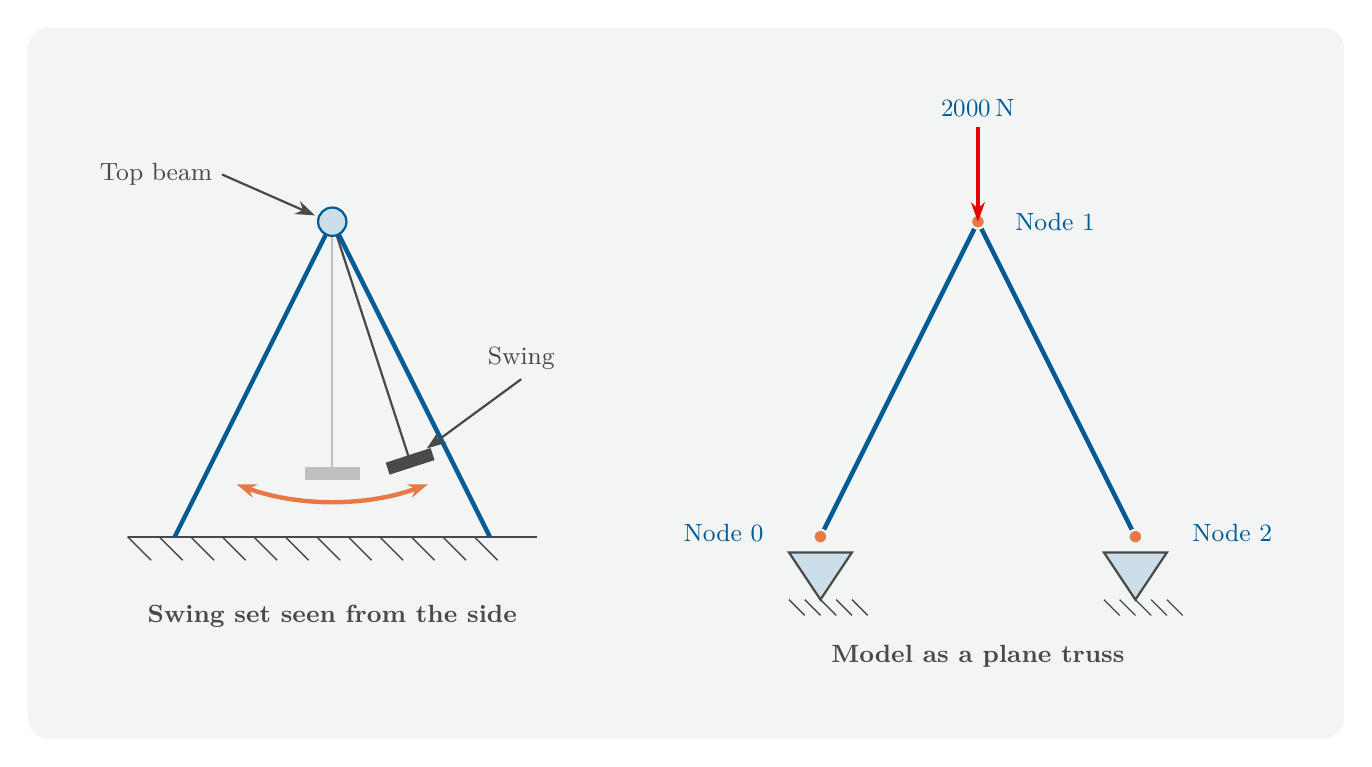
\begin{tikzpicture}[
    show background rectangle,
    background rectangle/.style={fill=my_lightgray, rounded corners=8pt},
    inner frame sep=0.8cm,
    annotation/.style={draw=my_darkgray, thick, -{Stealth[length=7pt, width=5pt]}}
]

    % Maßstab: 1 m = 2 cm. Knoten 0 (0,0), Knoten 1 (1 m, 2 m), Knoten 2 (2 m, 0)

    % ===== Panel 1: Schaukelgestell von der Seite =====
    \begin{scope}

        % Boden mit Schraffur
        \draw[draw=my_darkgray, thick] (-0.6,0) -- (4.6,0);
        \foreach \x in {-0.6,-0.2,...,4.2} {
            \draw[draw=my_darkgray, line width=0.5pt] (\x,0) -- ++(0.3,-0.3);
        }

        % Schaukel in Ruhelage (blass) und ausgelenkt um 18 Grad
        \draw[draw=my_darkgray!35, thick] (2,4) -- (2,0.8);
        \draw[fill=my_darkgray!35, draw=none]
            (1.65,0.72) rectangle (2.35,0.88);
        \draw[draw=my_darkgray, thick] (2,4) -- ($(2,4)+(-72:3.2)$);
        \draw[fill=my_darkgray, draw=none, rotate around={18:($(2,4)+(-72:3.2)$)}]
            ($(2,4)+(-72:3.2)+(-0.3,-0.08)$) rectangle
            ($(2,4)+(-72:3.2)+(0.3,0.08)$);

        % Schwingbewegung
        \draw[draw=my_orange, ultra thick, {Stealth[length=7pt, width=5pt]}-{Stealth[length=7pt, width=5pt]}]
            ($(2,4)+(-110:3.55)$) arc[start angle=-110, end angle=-70, radius=3.55];

        % Beine des Bocks
        \draw[draw=my_darkblue, ultra thick] (0,0) -- (2,4) -- (4,0);

        % Querstange im Schnitt
        \draw[fill=my_lightblue, draw=my_darkblue, thick] (2,4) circle (0.18);

        % Beschriftungen
        \draw[annotation] (0.6,4.6) -- (1.78,4.08);
        \node[font=\small, text=my_darkgray, anchor=east] at (0.6,4.6) {Top beam};
        \draw[annotation] (4.4,2.0) -- (3.2,1.12);
        \node[font=\small, text=my_darkgray, anchor=south] at (4.4,2.0) {Swing};

        \node[font=\small\bfseries, text=my_darkgray, anchor=north]
            at (2,-0.75) {Swing set seen from the side};
    \end{scope}

    % ===== Panel 2: Modell als ebenes Fachwerk =====
    \begin{scope}[xshift=8.2cm]

        \coordinate (N0) at (0,0);
        \coordinate (N1) at (2,4);
        \coordinate (N2) at (4,0);

        \draw[draw=my_darkblue, ultra thick] (N0) -- (N1) -- (N2);

        \foreach \P in {N0, N1, N2} {
            \draw[fill=my_orange, draw=my_lightgray, thick] (\P) circle (2.5pt);
        }

        % Festlager an Knoten 0 und Knoten 2
        \draw[fill=my_lightblue, draw=my_darkgray, thick]
            (-0.4,-0.2) -- (0.4,-0.2) -- (0,-0.8) -- cycle;
        \foreach \x in {-0.4,-0.2,0,0.2,0.4} {
            \draw[draw=my_darkgray, line width=0.5pt] (\x,-0.8) -- ++(0.2,-0.2);
        }
        \draw[fill=my_lightblue, draw=my_darkgray, thick]
            (4.4,-0.2) -- (3.6,-0.2) -- (4,-0.8) -- cycle;
        \foreach \x in {3.6,3.8,4.0,4.2,4.4} {
            \draw[draw=my_darkgray, line width=0.5pt] (\x,-0.8) -- ++(0.2,-0.2);
        }

        % Last an der Spitze
        \draw[draw=my_red, ultra thick, -{Stealth[length=7pt, width=5pt]}]
            ($(N1)+(0,1.2)$) -- (N1);
        \node[font=\small, text=my_darkblue, anchor=south]
            at ($(N1)+(0,1.2)$) {$2000\,\mathrm{N}$};

        \node[font=\small, text=my_darkblue, anchor=east]
            at ($(N0)+(-0.6,0.05)$) {Node 0};
        \node[font=\small, text=my_darkblue, anchor=west]
            at ($(N1)+(0.35,0)$) {Node 1};
        \node[font=\small, text=my_darkblue, anchor=west]
            at ($(N2)+(0.6,0.05)$) {Node 2};

        \node[font=\small\bfseries, text=my_darkgray, anchor=north]
            at (2,-1.25) {Model as a plane truss};
    \end{scope}

\end{tikzpicture}
\end{document}
